\documentclass[12pt]{ctexart} % Use 10pt or 9pt as the base size
\usepackage{xeCJK} % For CJK support
\usepackage{fontspec} % For font settings

\usepackage{amsmath}
\usepackage{cases}
\usepackage{graphicx}
\usepackage[margin=1in]{geometry}
\usepackage{fancyhdr}
\usepackage{titlesec}
\usepackage{setspace}
\usepackage{hyperref} % For clickable links in the table of contents
\usepackage{tocloft} % For customizing the table of contents

\geometry{a4paper}
\setstretch{1.25} % Set line spacing to 1.25

\pagestyle{plain}
\pagenumbering{arabic}
% Set main font for Latin text

\setCJKfamilyfont{SimHei}[BoldFont={SimHei-Bold}]{SimHei}
\setmainfont{Times New Roman}
% Set font for CJK text
\setCJKmainfont{SimSun} % For body text
\setCJKsansfont{SimHei} % For sans-serif text, often used for titles

% Redefine section, subsection, etc. fonts
\titleformat{\section}{\normalfont\Large\bfseries\CJKfontspec{SimHei}}{\thesection}{1em}{}
\titleformat{\subsection}{\normalfont\large\bfseries\CJKfontspec{SimHei}}{\thesubsection}{1em}{}


\title{
\CJKfontspec{SimHei}\Huge\bfseries 基于图卷积神经网络的商品共购网络分析 \\
\Large 《金融科技导论与实践》智能营销大作业报告
}

\author{混合2209    马宇恒  3220105015\\
混合2209    肖一鸣  3220105015}

\date{\today}

\begin{document}


\fancyfoot[C]{\thepage}

\maketitle

\renewcommand{\cftsecleader}{\cftdotfill{\cftdotsep}}
\tableofcontents
\newpage


\section{研究背景与意义}

图卷积神经网络（GCN）是一种重要而基础的图学习方式，在图的分类工作中表现出色\cite{kipf2017semi}，其优势如下：

\begin{enumerate}
    \item 可以处理各种不规则的无向图数据，如社交网络、推荐系统、生物信息学等，适应范围广。
    \item 只依赖较小规模的标签数据，就可以对整个图进行分类预测。
    \item 可以将节点的高维附加信息（Side Information）作为嵌入特征（Embedding Feature）投入训练，配合各种特征工程，可以提高模型的泛化能力。
\end{enumerate}


而商品共购网络（Co-purchasing Network）是智能营销领域中的一种重要图数据，通过收集被用户一次性同时购买的商品信息，搭建商品之间的关联网络。
而利用该网络，可以将商品按关联度聚类，构建商品列表，为各大网购平台中的 “顺手买一件”、“看了又看”（Customers Who Buy This Item Also Buy） 等功能提供策略支持，并在其他商品推荐、定价场景发挥作用，实现营销价值。

因此，利用 GCN 对商品共购网络进行分析，可以为智能营销领域提供新的思路和方法，为商品推荐、定价等场景提供更好的支持。

\section{国内外研究现状}

\subsection{ CGN 之前的工作}

早在二十世纪末期，就有卷积神经网络 （CNN） 的概念，但当时的卷积神经网络仅将 不同的滤波器 （Filter） 用于位图即规整的网格图，以采得不同尺度的特征，
但要将卷积应用于一般图数据，其难点在于一般图特征在不同尺度上的提取。

而拉普拉斯矩阵（Laplace matrix）由图的邻接矩阵 $A$ 导出，可以将其看作是一种图特征，表现了所有顶点的连通性，反映其该顶点位置为中心或离群。
未归一化和已经归一化的拉普拉斯矩阵 $L$ 表示如下，其中 $D$ 为度数矩阵，$A$ 为邻接矩阵：

\[
\begin{aligned}
    D_{ii} &= \sum_{j=1}^{N} A_{ij}, \quad \quad \quad
    L_{\text{unnormalized}} &= D - A , \quad \quad \quad
    L_{\text{normalized}} &= I_N - D^{-\frac{1}{2}} A D^{-\frac{1}{2}} .
\end{aligned}
\]

2016 年的一篇论文\cite{yang_revisiting_2016} 总结了在 GCN 之前的半监督图学习模型，
强调归一化拉普拉斯矩阵对于半监督学习的重要性，半将 $L$ 作为 Loss 的正则项以防止模型过平滑。
这也为后续的 GCN 模型直接将拉普拉斯矩阵作为 Forwarding 函数 提供了重要的参考。
并且，该论文首先提出了 Citeseer 引用网络数据集，用于测试半监督图学习模型的分类能力。


\subsection{ CGN 模型提出}


GCN 的研究始于 2017 年，由 Kipf 和 Welling 提出的 GCN 模型 \cite{kipf2017semi}，是一种基于图的半监督学习方法，可用于 Citeseer 数据集。
这篇论文使用拉普拉斯矩阵在本征空间上的不同缩放算子 $g_{\theta}$ 来实现不同尺度特征的提取。
通过该卷积操作，将节点的特征信息传递给邻居节点，从而实现节点之间的信息传递。

\[
g_{\theta}\star x=U g_{\theta}U^{T}x
\]


上述式子必须进一步化简，否则大型图的 $N$ 阶矩阵本征值分解将是无比耗时的。于是借助 2009 年 Hammond 等人提出的一种基于拉普拉斯矩阵的小波变换方法\cite{hammond_wavelets_2009}，
这项研究利用了切比雪夫多项式 （Chebyshev polynomial）在多项式 0-1 积分内积空间 $R^N[x]$ 上的正交性，
得到了用多项式近似缩放算子的方法：

\[
    g_{\theta^{\prime}}(\Lambda)\approx\sum_{k=0}^{K}\theta_{k}^{\prime}T_{k}(\tilde{\Lambda})
    \tag{1}
\]


接着是进一步消去 $\Lambda$ 和 $U$。我们假设无向图，即邻接矩阵 $A$ 是对称的；从而 $L$ 也是对称的正规矩阵。
由实谱定理（Spectral theorem）可知，在 $R^N$ 实空间中存在由 $L$ 的本征向量构成的标准正交基，
这使得其本征值分解 $L=U^T \Lambda U $ 中， $U$ 是酉矩阵（等距同构），满足 $ U^T U = I_N $。
从而有 $L^k = (U\Lambda U^{\top})^{k}=U\Lambda^{k}U^{\top}$ 。 这个等式说明，只需要使用关于 $L$ 的多项式，即可表示 (1) 式。

\[
    g_{\theta^{\prime}}\star x\approx\sum_{k=0}^{K}\theta_{k}^{\prime}T_{k}(\tilde{L})x
\]

最后结合 renormalize trick 提升节点自身的 embedding feature 的重要性，便得出了 GCN 最基础的前向传播公式：

\[
    Z=\tilde{D}^{-{\frac{1}{2}}}\tilde{A}\tilde{D}^{-{\frac{1}{2}}}X\Theta
\]



\subsection{局限与发展}


但 GCN 并非万能，也存在如下局限性：

\begin{itemize}
    \item GCN 由于直接将图的高维特征输入神经网络，并且在前向传播的过程中必须保存 $F_{l} \times N  + F_{l+1} \times N $的嵌入特征数据，这使得 GCN 训练过程中消耗较大内存，对于比较大型的图数据，会导致训练效率低下。
    \item GCN 的原理推导使用了无向图的假设，因此不能直接应用于有向图。而对于有向图数据，需要额外的处理，例如增加一倍的冗余节点，将原图改造为无向的二分图，但这也会带来性能开支的增大。
\end{itemize}


之后，GCN 发展出了不同的变体，以应对一般图学习中层出不穷的场景。例如，引入注意力机制的图神经网络 GAT 便适用于有向图； 使用采样和聚合的卷积网络算法 GraphSAGE，使其可扩展化，适用于更大规模的图数据。
而在实际应用场景中， GCN 卷积层也搭配其他神经网络层，如池化层， LSTM、GRU，普通线性全链接层等，以实现深度学习，提高模型的泛化能力。

因此，在本次实验中，我们尝试在 GCN 基础模型的基础上添加更多实际应用中的技巧，以提高模型的性能。
同时利用半监督数据的规模大小，探讨 GCN 在该模式下学习分类的极限训练数据大小。 在后续章节的实验中，我们将详细介绍我们的实验设计和结果分析。

\section{研究思路}

我们遵循从原理到应用、从基础到扩展顺序展开研究：

\begin{enumerate}
    \item 了解图神经网络原理， 学习论文和 \href{https://web.stanford.edu/class/cs224w/}{cs224w}  课程中对于 GNN 的相关介绍，以及
特征工程、网络搭建技巧，实现 Pytorch 版本的模型，并尽可能多地扩展可调参数。
    \item 利用著名的 Citeseer 引用网络数据集，对比实验数据和论文数据，验证代码正确性。
    \item 使用 Optuna 等超参数优化工具，对 GCN 模型的超参数进行调优，以提高模型的性能。
    \item 借助正确的模型，对商品共购网络进行分析，探讨该模型在商品推荐领域的分类表现。可视化商品共购网络，分析商品之间的关联性。
    \item 有了以上模型和实验结果，我们将进一步探讨 GCN 在半监督学习中的极限训练数据大小，得到该模型学习能力的更直观认识。
\end{enumerate}


首先，论文提供的是 tensorflow 版本的 GCN 模型\cite{kipf2017semi}，
为了匹配现有环境，我们将其改写为 PyTorch 版本。TODO


\section{论文引用网络分析}


\begin{figure}[h]
    \centering
    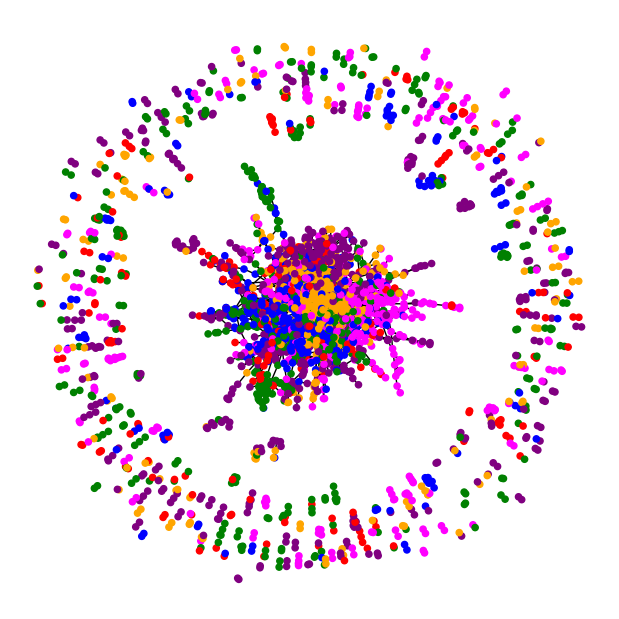
\includegraphics[width=0.6\textwidth]{assets/citeseer-adj.png}
    \caption{Your caption text goes here}
    \label{fig:example}
\end{figure}


\section{亚马逊共购网络分析}



\cite{hamilton_inductive_2018}

\cite{yang_revisiting_2016}
\cite{hammond_wavelets_2009}
\cite{zeiler_visualizing_2013}
\cite{yang_defining_2012}

\bibliographystyle{plain}
\bibliography{./report}  %bib文件名

\end{document}